%%%%%%%%%%%%%%%%%%%%%%%%%%%%%%%%%%%%

\section{条件付き確率}

%%%%%%%%%%%%%%%%%%%%%%%%%%%%%%%%%%%%

\subsection{分割表を用いた確率の探索}

%%%%%%%%%%%%%%%%%%%%%%%%%%%%%%%%%%%%

\begin{frame}
\frametitle{再発}

研究者たちは、コカイン慢性使用者72人を3つのグループに無作為に割り当てた：デシプラミン（抗うつ薬）、リチウム（コカインの標準治療）、プラセボ。研究結果を以下にまとめる。

{\small
\begin{center}
\begin{tabular}{l | c c | c}
			& 		& 再発 		&  \\
			& 再発あり	& なし	& 合計 \\
\hline
デシプラミン	& 10		& 14		& 24 \\
リチウム		& 18		& 6		& 24 \\
プラセボ		& 20		& 4		& 24 \\
\hline
合計			& 48		& 24		& 72
\end{tabular}
\end{center}
}

\ct{\webURL{http://www.oswego.edu/~srp/stats/2_way_tbl_1.htm}}

\end{frame}

%%%%%%%%%%%%%%%%%%%%%%%%%%%%%%%%%%%%

\begin{frame}

\dq{患者が再発しなかった確率は何か？}


{\small
\begin{center}
\begin{tabular}{l | c c | c}
			& 		& 再発 		&  \\
			& 再発あり	& なし	& 合計 \\
\hline
デシプラミン	& 10		& 14		& 24 \\
リチウム		& 18		& 6		& 24 \\
プラセボ		& 20		& 4		& 24 \\
\hline
合計			& 48		& 24		& 72
\end{tabular}
\end{center}
}

\end{frame}

%%%%%%%%%%%%%%%%%%%%%%%%%%%%%%%%%%%%

\subsection{周辺確率と結合確率}

%%%%%%%%%%%%%%%%%%%%%%%%%%%%%%%%%%%%

\begin{frame}
\frametitle{周辺確率}

\dq{患者が再発した確率は何か？}

{\small
\begin{center}
\begin{tabular}{l | c c | c}
			& 		& 再発 		&  \\
			& 再発あり	& なし	& 合計 \\
\hline
デシプラミン	& 10		& 14		& 24 \\
リチウム		& 18		& 6		& 24 \\
プラセボ		& 20		& 4		& 24 \\
\hline
合計			& \red{48}		& 24		& \red{72}
\end{tabular}
\end{center}
}

P(再発あり) = $\frac{48}{72} \approx 0.67$ \\

\end{frame}

%%%%%%%%%%%%%%%%%%%%%%%%%%%%%%%%%%%%

\begin{frame}
\frametitle{結合確率}

\dq{患者が抗うつ薬（デシプラミン）を投与された\underline{かつ}再発した確率は何か？}

{\small
\begin{center}
\begin{tabular}{l | c c | c}
			& 		& 再発 		&  \\
			& 再発あり	& なし	& 合計 \\
\hline
デシプラミン	& \red{10}		& 14		& 24 \\
リチウム		& 18		& 6		& 24 \\
プラセボ		& 20		& 4		& 24 \\
\hline
合計			& 48	& 24		& \red{72}
\end{tabular}
\end{center}
}

P(再発あり かつ デシプラミン) = $\frac{10}{72} \approx 0.14$ \\

\end{frame}

%%%%%%%%%%%%%%%%%%%%%%%%%%%%%%%%%%%%

\subsection{条件付き確率の定義}

%%%%%%%%%%%%%%%%%%%%%%%%%%%%%%%%%%%%

\begin{frame}[shrink=10]
\frametitle{条件付き確率}

\formula{条件付き確率}{
条件 $B$ のもとで目的の結果 $A$ が起こる条件付き確率は次のように計算される
\[ P(A|B) = \frac{P(A~\text{かつ}~B)}{P(B)} \]
}

\twocol{0.5}{0.5}
{
{\small
\begin{center}
\begin{tabular}{l | c c | c}
			& 		& 再発 		&  \\
			& 再発あり	& なし	& 合計 \\
\hline
デシプラミン	& 10		& 14		& 24 \\
リチウム		& 18		& 6		& 24 \\
プラセボ		& 20		& 4		& 24  \\
\hline
合計			& 48		& 24		&  72
\end{tabular}
\end{center}
}
}
{
\begin{eqnarray*}
&&P(\text{再発} |  \text{デシプラミン}) \\
&&= \frac{P(\text{再発} ~ \text{かつ} ~ \text{デシプラミン})}{P(\text{デシプラミン})} \\
&&= \frac{10 / 72}{24 / 72} \\
&&= \frac{10}{24} \\
&&= 0.42
\end{eqnarray*}
}

\end{frame}

%%%%%%%%%%%%%%%%%%%%%%%%%%%%%%%%%%%%

\begin{frame}
\frametitle{条件付き確率（続き）}

\dq{患者が抗うつ薬（デシプラミン）を投与されたとわかっている場合、再発した確率は何か？}

{\small
\begin{center}
\begin{tabular}{l | c c | c}
			& 		& 再発 		&  \\
			& 再発あり	& なし	& 合計 \\
\hline
\rowcolor[gray]{.7}
デシプラミン	& \red{10}			& 14		& \red{24} \\
リチウム		& 18		& 6		& 24 \\
プラセボ		& 20 		& 4		& 24  \\
\hline
合計			& 48	& 24		&  72
\end{tabular}
\end{center}
}

P(再発 $|$ デシプラミン) = $\frac{10}{24} \approx 0.42$ \\

$\:$ \\
P(再発 $|$ リチウム) = $\frac{18}{24} \approx 0.75$ \\
P(再発 $|$ プラセボ) = $\frac{20}{24} \approx 0.83$ \\

\end{frame}

%%%%%%%%%%%%%%%%%%%%%%%%%%%%%%%%%%%%

\begin{frame}
\frametitle{条件付き確率（続き）}

\dq{患者が再発したとわかっている場合、抗うつ薬（デシプラミン）を投与されていた確率は何か？}

{\small
\begin{center}
\begin{tabular}{l | >{\columncolor[gray]{0.7}[0pt]}c c | c}
			& 		& 再発 		&  \\
			& 再発あり	& なし	& 合計 \\
\hline
デシプラミン	& \red{10}			& 14		& 24 \\
リチウム		& 18		& 6		& 24 \\
プラセボ		& 20		& 4		& 24  \\
\hline
合計			& \red{48}	& 24		&  72
\end{tabular}
\end{center}
}

P(デシプラミン $|$ 再発) = $\frac{10}{48} \approx 0.21$ \\

$\:$ \\
P(リチウム $|$ 再発) = $\frac{18}{48} \approx 0.375$ \\
P(プラセボ $|$ 再発) = $\frac{20}{48} \approx 0.42$ \\

\end{frame}

%%%%%%%%%%%%%%%%%%%%%%%%%%%%%%%%%%%%

\subsection{一般乗法定則}

%%%%%%%%%%%%%%%%%%%%%%%%%%%%%%%%%%%%

\begin{frame}
\frametitle{一般乗法定則}

\begin{itemize}

\item 2つの事象が独立である場合、その結合確率は単純にそれぞれの確率の積であることを見た。事象が独立でないと考えられる場合、結合確率は少し異なる方法で計算される。

\item $A$ と $B$ が2つの結果または事象を表す場合、
\formula{\[ P(A~\text{かつ}~B) = P(A|B) \times P(B) \]}
この式は、条件付き確率の公式を変形したものに過ぎない。

\item $A$ を目的の結果、$B$ を条件として考えると便利である。

\end{itemize}

\end{frame}

%%%%%%%%%%%%%%%%%%%%%%%%%%%%%%%%%%%%

\subsection{条件付き確率における独立性の考慮}

%%%%%%%%%%%%%%%%%%%%%%%%%%%%%%%%%%%%

\begin{frame}[shrink=10]
\frametitle{独立性と条件付き確率}

以下は、入門統計学クラスの学生の性別と専攻の（仮想の）分布である：

{\small
\begin{center}
\begin{tabular}{l | c c | c}
			& 社会	& 非社会 		&  \\
			& 科学	& 科学	& 合計 \\
\hline
女性		& 30		& 20		& 50 \\
男性			& 30		& 20		& 50 \\
\hline
合計			& 60		& 40		& 100
\end{tabular}
\end{center}
}

\begin{itemize}

\item 無作為に選ばれた学生が社会科学専攻である確率は $\frac{60}{100} = 0.6$。

\item 無作為に選ばれた学生が女性であるとわかっている場合、社会科学専攻である確率は $\frac{30}{50} = 0.6$。

\item $P(SS | M)$ も 0.6 に等しいため、このクラスの学生の専攻は性別に依存しない：P(SS $|$ F) = P(SS)。

\end{itemize}

\end{frame}

%%%%%%%%%%%%%%%%%%%%%%%%%%%%%%%%%%%%

\begin{frame}
\frametitle{独立性と条件付き確率（続き）}

一般的に、$P(A|B) = P(A)$ であれば、事象 $A$ と $B$ は独立であるといわれる。

\begin{itemize}

\item 概念的に：$B$ を与えても $A$ について何も教えてくれない。

\item 数学的に：事象 $A$ と $B$ が独立であれば $P(A~\text{かつ}~B) = P(A) \times P(B)$ であることがわかっている。すると、
\[ P(A|B) = \frac{P(A~\text{かつ}~B)}{P(B)} = \frac{P(A) \times P(B)}{P(B)} = P(A) \]

\end{itemize}

\end{frame}

%%%%%%%%%%%%%%%%%%%%%%%%%%%%%%%%%%%%

\subsection{樹形図}

%%%%%%%%%%%%%%%%%%%%%%%%%%%%%%%%%%%%

\begin{frame}[shrink=25]
\frametitle{乳がん検診}

\begin{itemize}

\item 米国がん協会の推定によれば、女性の約1.7\%が乳がんを患っている。 \\
{\small\webURL{http://www.cancer.org/cancer/cancerbasics/cancer-prevalence}}

\item Susan G. Komen For The Cure Foundation によれば、マンモグラフィは実際に乳がんを患っている女性の約78\%を正確に識別する。 \\
{\small\webURL{http://ww5.komen.org/BreastCancer/AccuracyofMammograms.html}}

\item 2003年に発表された論文によれば、すべてのマンモグラフィのうち最大10\%ががんを患っていない患者に対して偽陽性を示す。 \\{\small \webURL{http://www.ncbi.nlm.nih.gov/pmc/articles/PMC1360940}}

\end{itemize}

\vfill

\Note{これらの割合は近似値であり、推定が非常に難しい。}

\end{frame}

%%%%%%%%%%%%%%%%%%%%%%%%%%%%%%%%%%%

\begin{frame}[shrink=10]
\frametitle{確率の逆転}

\dq{患者が乳がん検診を受けるとき、2つの競合する主張がある：患者はがんである、患者はがんでない。マンモグラフィが陽性の結果を示した場合、患者が実際にがんである確率は何か？}

\twocol{0.7}{0.3}{
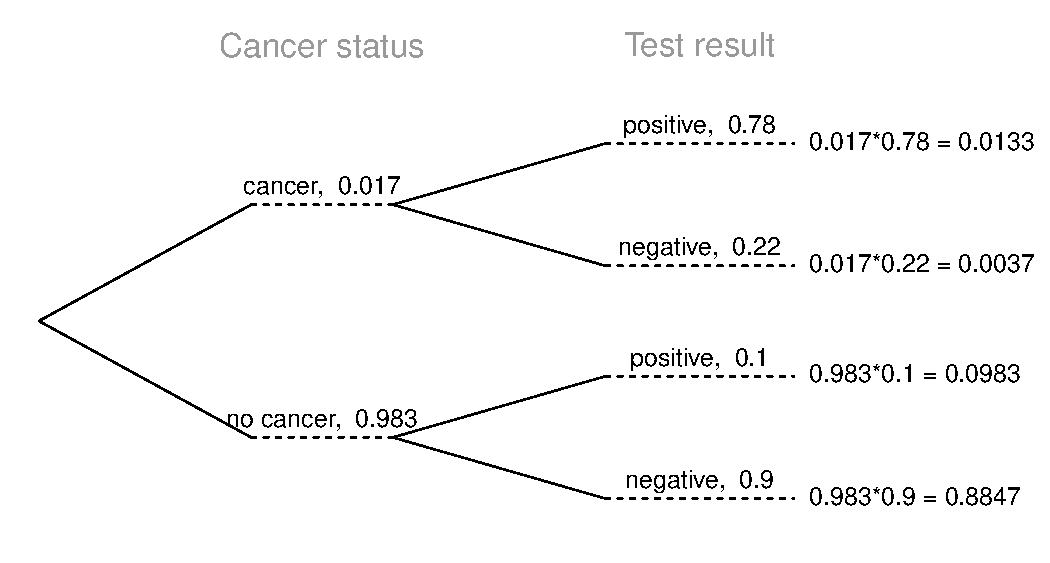
\includegraphics[width=\textwidth]{3-2_conditional_probability/figures/cancer_tree/cancer_tree_first}
}
{
{\footnotesize
\begin{eqnarray*}
&&P(C | +) \\
&&= \frac{P(C~\text{かつ}~+)}{P(+)} \\
&&= \frac{0.0133}{0.0133 + 0.0983} \\
&&= 0.12
\end{eqnarray*}
}
}

\Note{樹形図は確率を逆転させるのに有用である：$P(+|C)$ が与えられ、$P(C|+)$ を求める。}

\end{frame}

%%%%%%%%%%%%%%%%%%%%%%%%%%%%%%%%%%%

\begin{frame}
\frametitle{練習問題}

\pq{1回検査を受けて陽性の結果を得た女性が再検査を受けたいとする。2回目の検査では、この特定の女性ががんである確率はいくつと仮定すべきか？}

\begin{enumerate}[(a)]
\item 0.017
\solnMult{0.12}
\item 0.0133
\item 0.88
\end{enumerate}

\end{frame}

%%%%%%%%%%%%%%%%%%%%%%%%%%%%%%%%%%%

\begin{frame}
\frametitle{練習問題}

\pq{この2回目のマンモグラフィでも陽性の結果が出た場合、この女性ががんである確率は何か？}

\twocol{0.2}{0.7}
{
\begin{enumerate}[(a)]
\item 0.0936
\item 0.088
\item 0.48
\solnMult{0.52}
\end{enumerate}
}
{
\solnGr{
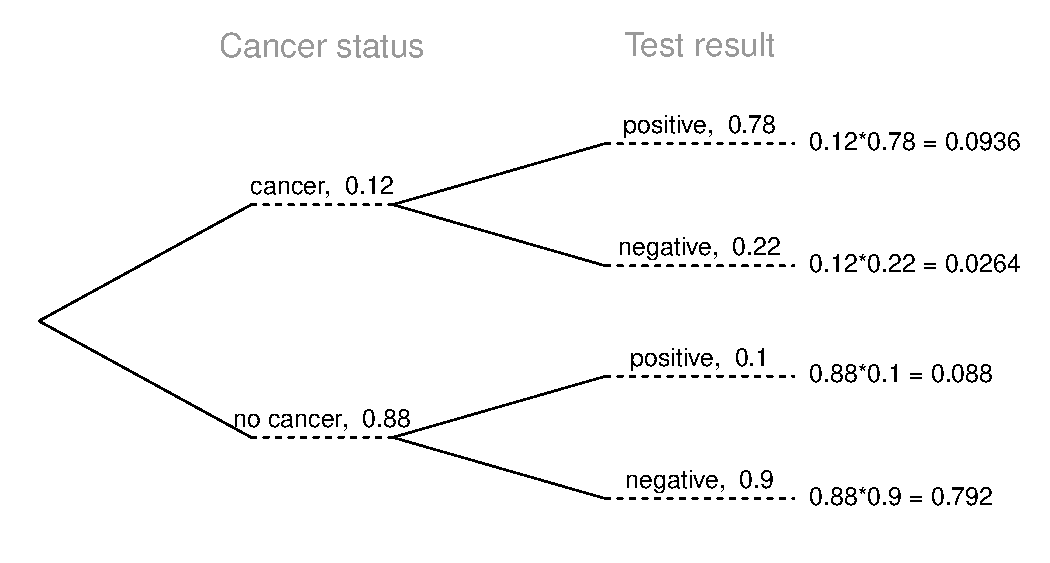
\includegraphics[width=\textwidth]{3-2_conditional_probability/figures/cancer_tree/cancer_tree_second}
}
}

\soln{
{\small \[P(C | +) = \frac{P(C~\text{かつ}~+)}{P(+)} = \frac{0.0936}{0.0936+0.088} = 0.52\]}
}

\end{frame}

%%%%%%%%%%%%%%%%%%%%%%%%%%%%%%%%%%%

\subsection{ベイズの定理}

%%%%%%%%%%%%%%%%%%%%%%%%%%%%%%%%%%%%

\begin{frame}
\frametitle{ベイズの定理}

\begin{itemize}

\item これまで見てきた条件付き確率の公式は、ベイズの定理の特殊な場合であり、事象が2つ以上の結果を持つ場合にも適用できる。

\item \hl{ベイズの定理：}
\formula{
\[ P(\text{変数1の結果}~A_1~|~\text{変数2の結果}~B) \]
\[ = \frac{P(B|A_1)P(A_1)}{P(B|A_1)P(A_1) + P(B|A_2)P(A_2) + \cdots + P(B|A_k)P(A_k)} \]
}
ここで $A_2$, $\cdots$, $A_k$ は変数1のその他のすべての可能な結果を表す。

\end{itemize}

\end{frame}

%%%%%%%%%%%%%%%%%%%%%%%%%%%%%%%%%%%

\begin{frame}
\frametitle{応用活動：確率の逆転}

\app{{\footnotesize 疾病の拡散を表す一般的な疫学モデルとして SIR モデルがある。このモデルでは、人口が感受性（Susceptible）、感染（Infected）、回復（Recovered）の3つのグループに分けられる。これは、1回の感染が通常その後の感染に対する免疫を与える水痘のような疾患に対して合理的なモデルである。これらの疾患は検出が難しいこともある。 \vspace{2mm} \\
人口の60\%が感受性、10\%が感染、30\%が回復状態にある疫病の最中の人口を想像する。この疾患の唯一の検査は、感受性者に対して95\%、感染者に対して99\%、回復者に対して65\%の精度を持つ。（注：ここで精度とは、感受性者と回復者に対して陰性、感染者に対して陽性の結果を返すことを意味する）。 \vspace{2mm} \\
上記の情報を反映した確率樹を描きなさい。個人が陽性と検査された場合、実際に感染している確率は何か？
}}

\end{frame}

%%%%%%%%%%%%%%%%%%%%%%%%%%%%%%%%%%%

\begin{frame}[shrink=15]
\frametitle{応用活動：確率の逆転（続き）}

\vspace{-0.5cm}

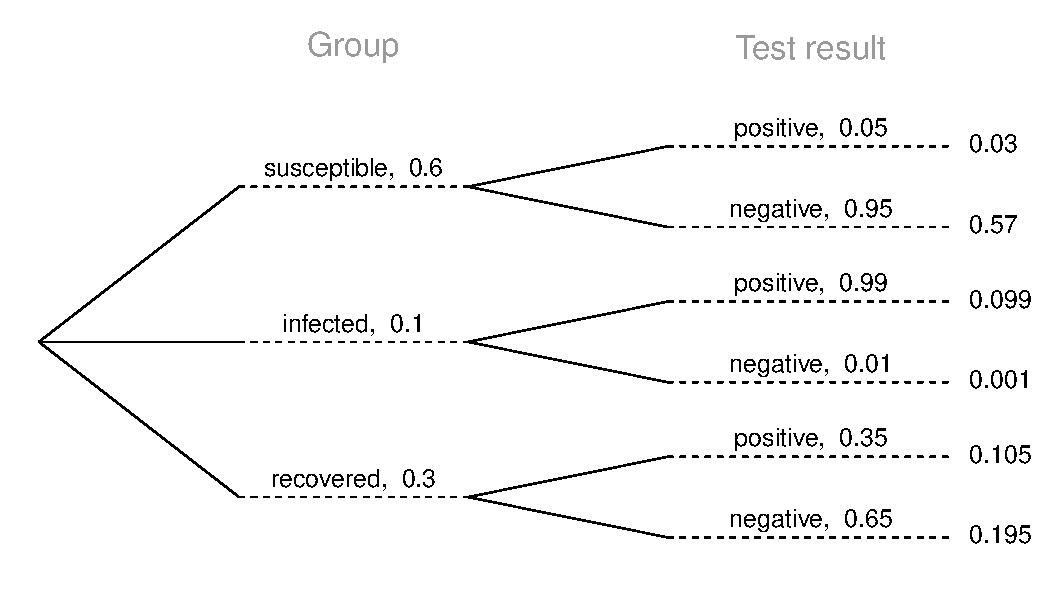
\includegraphics[width=\textwidth]{3-2_conditional_probability/figures/sir_tree/sir_tree}

\[ P(\text{感染} | +) = \frac{P(\text{感染}~\text{かつ}~+)}{P(+)} = \frac{0.099}{0.03 + 0.099 + 0.105} \approx 0.423 \]


\end{frame}

%%%%%%%%%%%%%%%%%%%%%%%%%%%%%%%%%%%%
